\section{Sensitivity of \texorpdfstring{$\omega_{a}$}{} to gain corrections}
\label{Sec:SystematicGain}

	I estimate the systematic error on R due to the the in-fill gain function at 24.8 ppb, and to the Short Term Double Pulse correction at blank ppb. Adding these in quadrature results in a systematic error of blank ppb.

	\subsection{In-Fill Gain}

		As positrons hit the calorimeters throughout the fill, there will be a gain sag response such that the energy of detected positrons changes throughout the fill, dropping at first and then rising exponentially back up to their true values. This changing energy response will lead to a systematic error on R, as positrons with mis-measured energies near the energy threshold are excluded from the fit. This gain sag is corrected for in the Recon West code, before I fill my histograms. Due to the way I've constructed my analysis code, it's not so simple to modify the reconstruction code and create new histograms quickly. Such a process would require the rebuilding of many sets of new cluster root trees, and then making histograms from those. As a faster way of getting at the in fill gain systematic error, I've instead chosen to apply a gain sag function to the incoming energy-corrected clusters. This allows me to scan over gain sag function parameters and only run off one set of trees, as I've been doing for all systematic studies.

		(Should this bit be in the analysis procedures chapter?) The in-fill gain sag function was determined by Matthias Smith and the laser team as shown in \DB{14077}. (Cite or link?) The function goes as  
			\begin{gather}
				E = E_{0}(1 - A \cdot e^{-(t-t_{offset})/\tau}),
			\label{Eqn:GainSag}
			\end{gather}
		where $E_{0}$ is the orginal energy of the positron cluster, A is the amplitude factor on the gain sag function, $\tau$ the lifetime, and then $t_{offset}$ the shift of the function from 0. It is this function that is inverted and applied to the clusters in the reconstruction. I apply a function of the same form in my own code before filling hits into histograms, in essence undoing the reconstruction gain correction as a way to measure the in-fill gain sag effect on R.

		\begin{figure}[h]
			\centering
			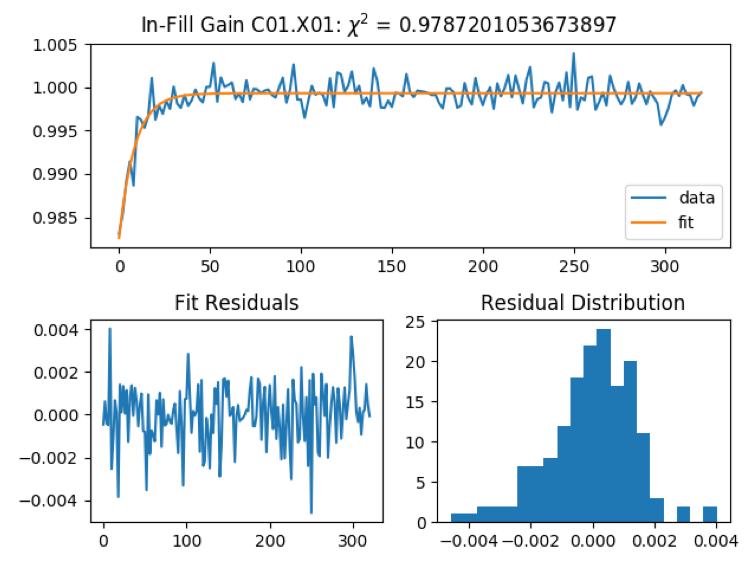
\includegraphics[width=.8\textwidth]{MatthiasInFill}
		    \caption[MatthiasInFill]{The top plot shows the in-fill gain sag function in orange from a fit to data in blue, for crystal 1 in calorimeter 1. The gain sag can be modeled effectively by a simple exponential function. By $\SI{30}{\mu s}$ the change in energy response is nearly only .1\%. (Might want to look up these exact numbers.) The bottom two plots show the residuals of the fit. Plot made by Matthias Smith.}
		    \label{Fig:MatthiasInFill}
		\end{figure}

		There are some simplifications and assumptions I've made when applying said gain sag function in my own code. First is that while in the reconstruction code each crystal of each calorimeter has its own singular in-fill gain function, one of which is shown in Figure \ref{Fig:MatthiasInFill}, I apply a global gain sag function to all incoming clusters. Secondly the default parameters for the gain sag function are simply eyeballed from the fcl file where all crystal parameters are stored. These values are 0.03 for the amplitude, $\SI{6.7}{\mu s}$ for the lifetime, and $\SI{3.907}{\mu s}$ for the offset. (Once the latest dataset is available I will need to come up with a better way to apply this gain sag function, either with multiple functions per crystal or with parameters that are actual averages. For now it's fine though to get words on the paper.) Finally, I apply this gain sag function after I apply the artificial deadtime to the incoming clusters, due to code restrictions. This should be a small effect. These assumptions I believe should be okay as long as I take my systematic errors conservatively.

		\begin{figure}[]
		\centering
		    \begin{subfigure}[t]{0.45\textwidth}
			    \centering
				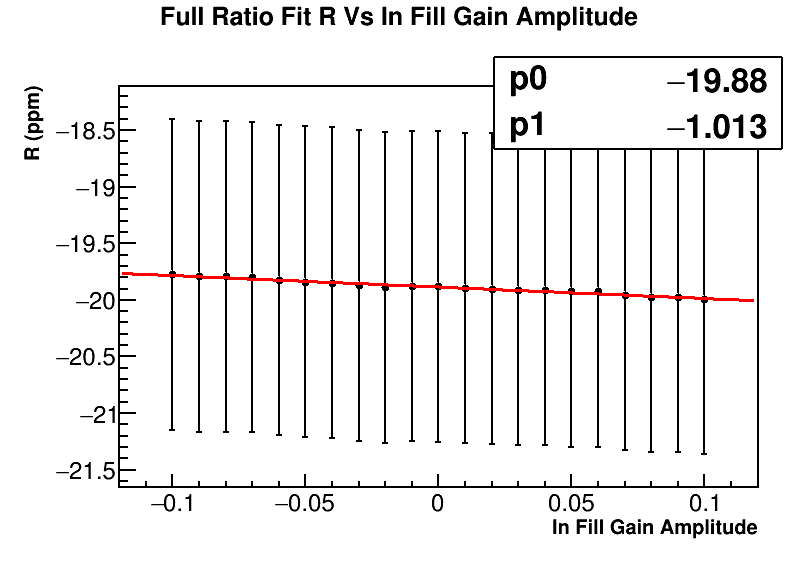
\includegraphics[width=\textwidth]{RatioCBO_R_Vs_InFillGainAmplitude_Canv}
			    \caption{Plotted is R vs the amplitude parameter in the gain sag function. The slope is -1.013 ppm per unit amplitude.}
		    \end{subfigure}
		    \hspace{4mm}
		    \begin{subfigure}[t]{0.45\textwidth}
			    \centering
				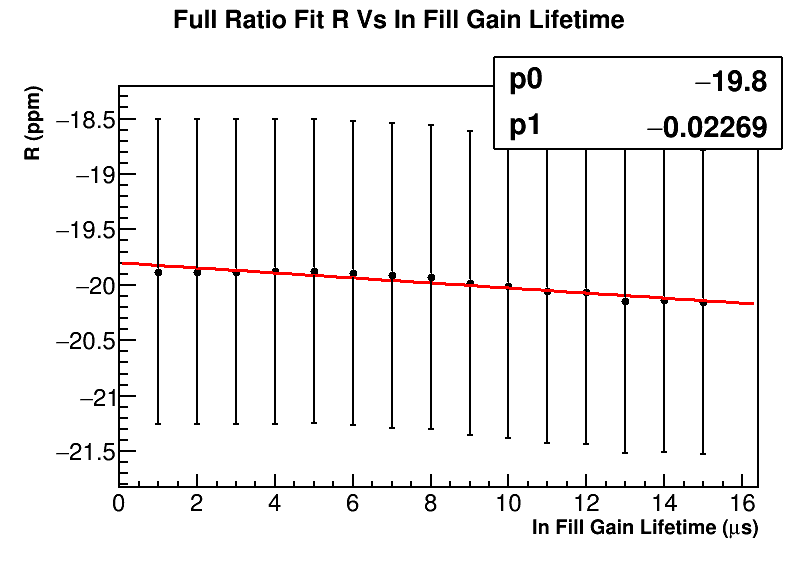
\includegraphics[width=\textwidth]{RatioCBO_R_Vs_InFillGainLifetime_Canv}
			    \caption{Plotted is R vs the lifetime parameter in the gain sag function. The slope is -0.02269 ppm per $\mu s$.}
		    \end{subfigure}% %you need this % here to add spacing between subfigures
		    \vspace{4mm}
		    \begin{subfigure}[t]{0.45\textwidth}
			    \centering
				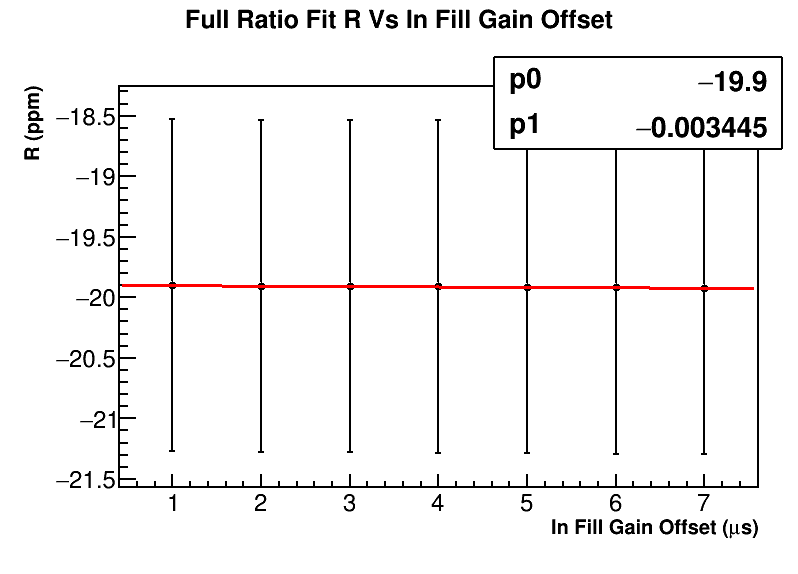
\includegraphics[width=\textwidth]{RatioCBO_R_Vs_InFillGainOffset_Canv}
			    \caption{Plotted is R vs the offset parameter in the gain sag function. The slope is -0.0034 ppm per $\mu s$.}
		    \end{subfigure}% %you need this % here to add spacing between subfigures
		\caption[InFillGain]{Plotted is fitted R values vs gain sag function parameters. In each case I scanned over ranges approximately centered around the eyeballed average values.}
		\label{Fig:InFillGain}
		\end{figure}

		To calculate the systematic error, I simply scan over the gain sag function parameters and observe the changes in R. This includes scans over the amplitude, lifetime, and offset as described in \ref{Eqn:GainSag}, and shown in Figure \ref{Fig:InFillGain}. I calculate the systematic error on R as the quadrature sum of the separate pieces as 
		\begin{align}
			\delta R_{A} &= \delta\alpha_{A} \times \frac{dR}{d\alpha_{A}}, \\
			\delta R_{\tau} &= \delta\alpha_{\tau} \times \frac{dR}{d\alpha_{\tau}}, \\
			\delta R_{offset} &= \delta\alpha_{offset} \times \frac{dR}{d\alpha_{offset}},
		\end{align}
		where $\delta\alpha_{A}$, $\delta\alpha_{\tau}$, and $\delta\alpha_{offset}$ are the uncertainties on the gain sag amplitude, lifetime, and offset respectively. I take the uncertainty on the amplitude very conservatively at 1\%, leading to a systematic error on R of $0.01 \times \SI{1.013}{ppm} = \SI{10.1}{ppb}$. I take the uncertainty on the lifetime very conservatively at $\SI{1}{\mu s}$, leading to a systematic error on R of $1 \times \SI{22.7}{ppb} = \SI{22.7}{ppb}$. Finally the slope for the offset parameter is very flat, and that combined with a very uniform array of values for the offset parameter in the reconstruction (indicative of a very small uncertainty), means that the systematic error on R is negligible. Therefore I ignore the offset parameter and add the amplitude and lifetime errors in quadrature to produce a systematic error on R of 24.8 ppb. (The uncertainty on the parameters would be the fit errors on the parameter I think, except for the fact that I'm using a global gain sag function as opposed to crystal functions, meaning the uncertainty might be the spread in parameters. I'm not entirely sure. Also I have removed the offset parameter in my latest code and will reproduce these results without it with the new dataset when it's available.)
